% Appendix A

\chapter{Arquitectura de la red y Resultados obtenidos} % Main appendix title

\label{AppendA} % For referencing this appendix elsewhere, use \ref{AppendixA}
\section{Capas de la red neuronal convolucional}

\begin{figure}[H]
		\begin{center}
		\begin{tikzpicture}[node distance=2cm]
		\node (input) [startstop] {Capa de Entrada};
		\node (conv1) [startstop, below of=input] {Capa de convolución 1};
		
		\node (pool1) [startstop, below of=conv1] {Capa Pooling 1};
		\node (conv2) [startstop, below of=pool1] {Capa de convolución 2};
		\node (pool2) [startstop, below of=conv2] {Capa Pooling 2};
		\node (full) [startstop, below of=conv2] {Full Layer};
		\node (exit) [startstop, below of=full] {Capa de salida};
		\draw [arrow] (input) -- (conv1) ;
		\draw [arrow] (conv1) -- (pool1);
		\draw [arrow] (pool1) -- (conv2);
		\draw [arrow] (conv2) -- (pool2);
		\draw [arrow] (pool2) -- (full);
		\draw [arrow] (full) -- (exit);
		\end{tikzpicture}
	\end{center}
	\caption{Capas de la red neuronal usada \\ Fuente:  \textit{Fuente Propia}}
\end{figure}



\section{Resultados de precisión de entrenamiento}
\subsection{CIFAR-10}
\begin{figure}[H]
	\begin{centering}
		\subfloat[fig 1]{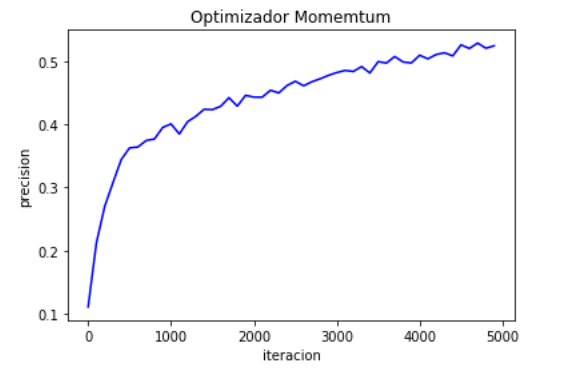
\includegraphics[width=0.45\textwidth]{Figures/momemtum5000.png}} 
		\subfloat[fig 2]{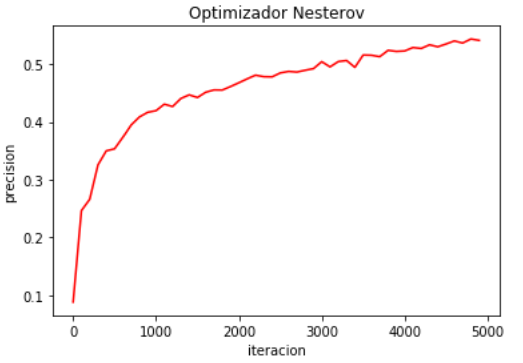
\includegraphics[width=0.45\textwidth]{Figures/nesterov5000.png}}\\
		\subfloat[fig 3]{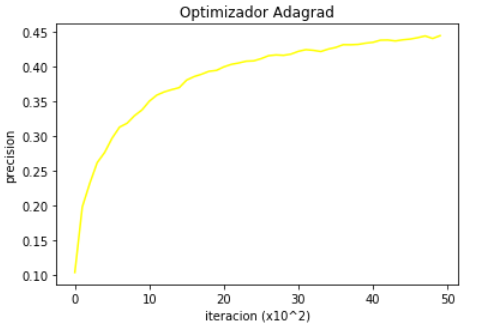
\includegraphics[width=0.45\textwidth]{Figures/adagrad5000.png}}
		\subfloat[fig 3]{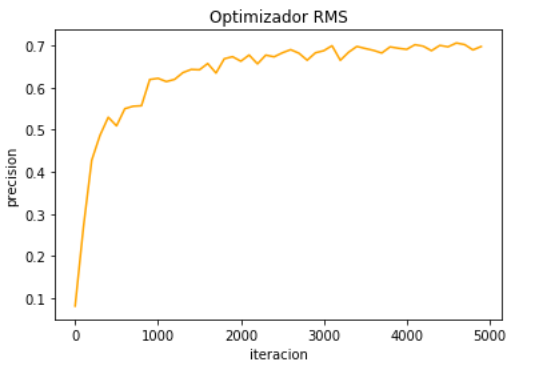
\includegraphics[width=0.45\textwidth]{Figures/rms5000.png}}\\
		\subfloat[fig 4]{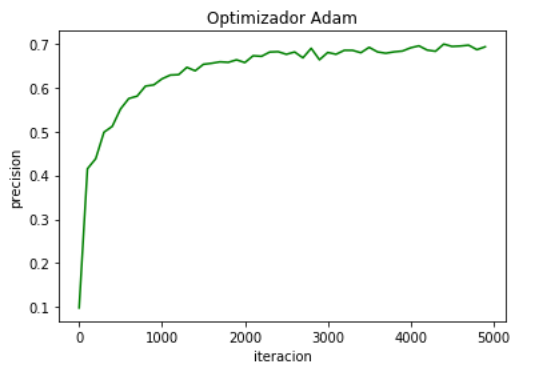
\includegraphics[width=0.5\textwidth]{Figures/adam5000.png}} 
		\caption{optmizadores 5000 epochs \\ Fuente :{\textit{Fuente Propia}}}
		\label{some example0}
	\end{centering}

\end{figure}


\begin{figure}[H]
	\begin{centering}
		\subfloat[fig 1]{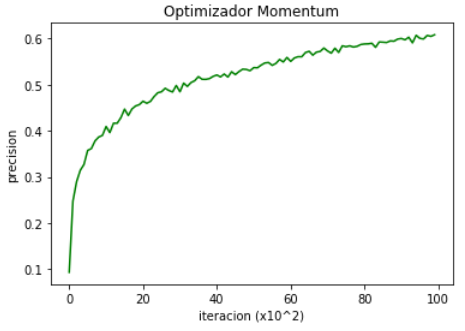
\includegraphics[width=0.55\textwidth]{Figures/momemtum10000.png}} 
		\subfloat[fig 2]{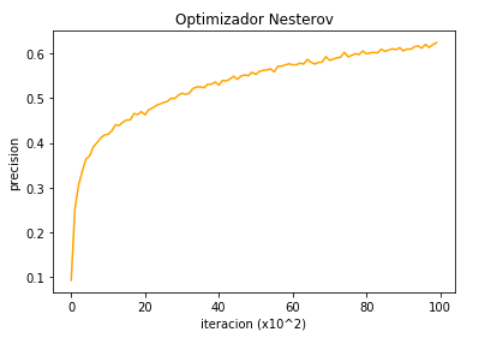
\includegraphics[width=0.55\textwidth]{Figures/nesterov10000.png}}\\
		\subfloat[fig 3]{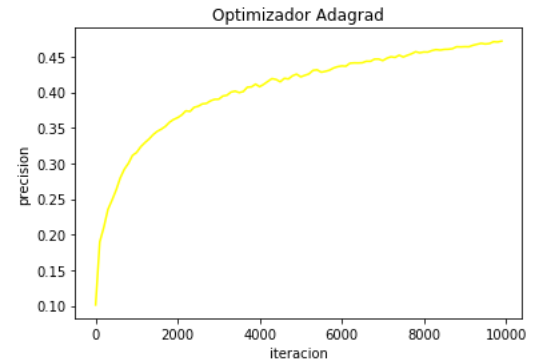
\includegraphics[width=0.55\textwidth]{Figures/adagrad10000.png}}
		\subfloat[fig 3]{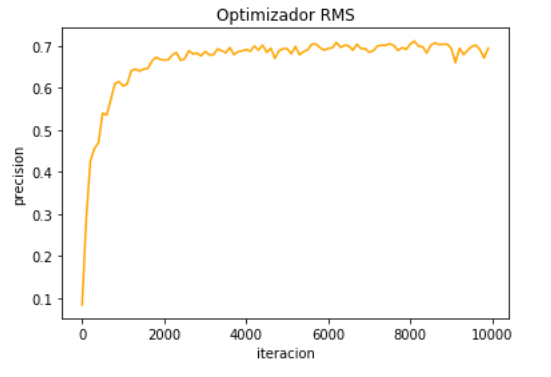
\includegraphics[width=0.55\textwidth]{Figures/rms10000.png}}\\
		\subfloat[fig 4]{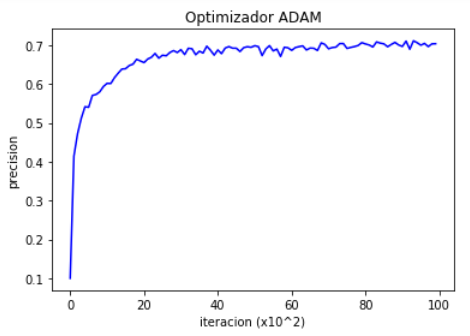
\includegraphics[width=0.6\textwidth]{Figures/adam10000.png}} 
		\caption{optmizadores 10000 epochs\\ Fuente:  \textit{Fuente Propia}}
		\label{some example1}
	\end{centering}
	
\end{figure}

\begin{figure}[H]
	\begin{centering}
		\subfloat[fig 1]{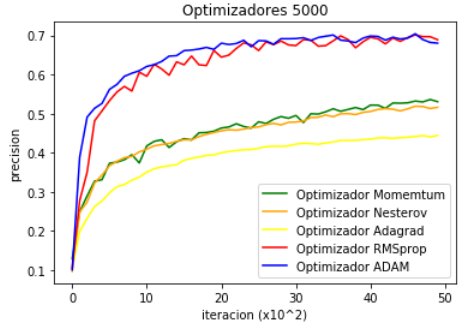
\includegraphics[width=0.8\textwidth]{Figures/optimizadores5000.png}} 
		\caption{Comparación de precisión de optimizadores para 5000 epochs\\ Fuente:  \textit{Fuente Propia}}
		\label{some example2}
	\end{centering}
	
\end{figure}

\begin{figure}[H]
	\begin{centering}
		\subfloat[fig 1]{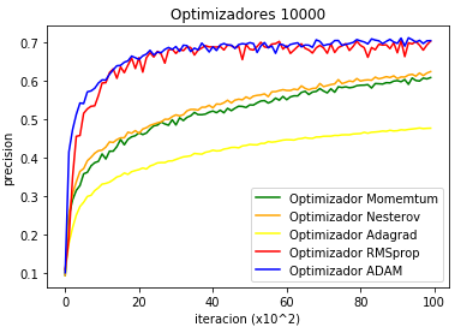
\includegraphics[width=0.8\textwidth]{Figures/optimizadores10000.png}} 
		\caption{Comparación de optimizadores para 10000 epochs\\ Fuente:  \textit{Fuente Propia}}
		\label{some example3}
	\end{centering}
	
\end{figure}

\subsection{CIFAR-100}

\begin{figure}[H]
	\begin{centering}
		\subfloat[fig 1]{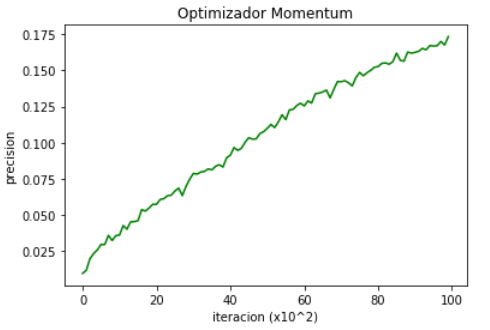
\includegraphics[width=0.55\textwidth]{Figures/100momemtum10000.png}} 
		\subfloat[fig 2]{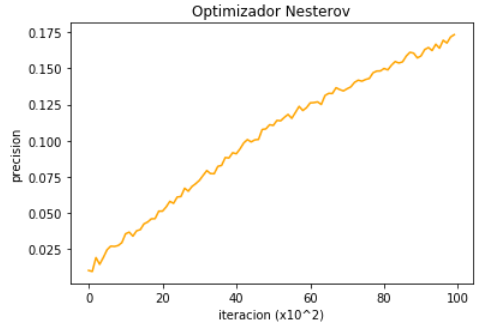
\includegraphics[width=0.55\textwidth]{Figures/100nesterov10000.png}}\\
		\subfloat[fig 3]{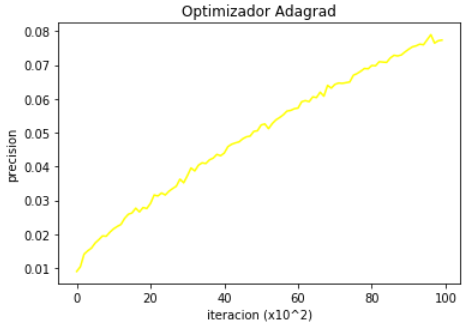
\includegraphics[width=0.55\textwidth]{Figures/100adagrad10000.png}}
		\subfloat[fig 3]{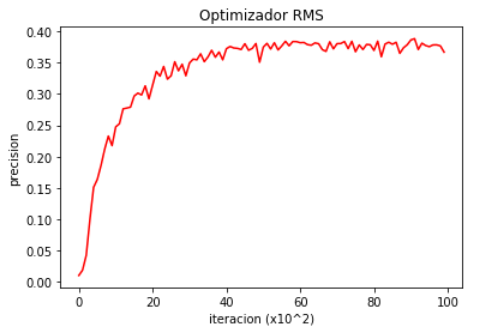
\includegraphics[width=0.55\textwidth]{Figures/100rms10000.png}}\\
		\subfloat[fig 4]{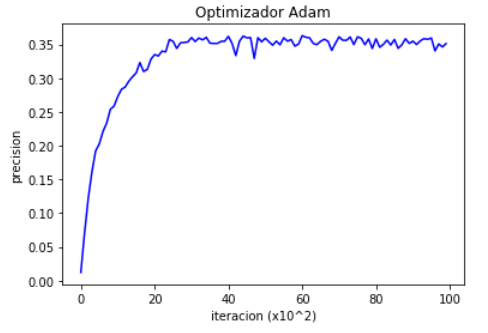
\includegraphics[width=0.6\textwidth]{Figures/100adam10000.png}} 
		\caption{optmizadores 10000 epochs\\ Fuente:  \textit{Fuente Propia}}
		\label{some exampleasa1}
	\end{centering}
	
\end{figure}



\begin{figure}[H]
	\begin{centering}
		\subfloat[fig 1]{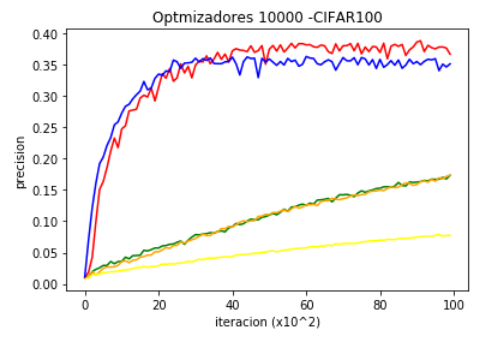
\includegraphics[width=0.8\textwidth]{Figures/cifar100result.png}} 
		\caption{Comparación de optimizadores para 10000 epochs - CIFAR100\\ Fuente:  \textit{Fuente Propia}}
		\label{some example32}
	\end{centering}
	
\end{figure}
\section{Resultados del error en el entrenamiento}
\subsection{CIFAR-10}
\begin{figure}[H]
	\begin{centering}
		\subfloat[fig 1]{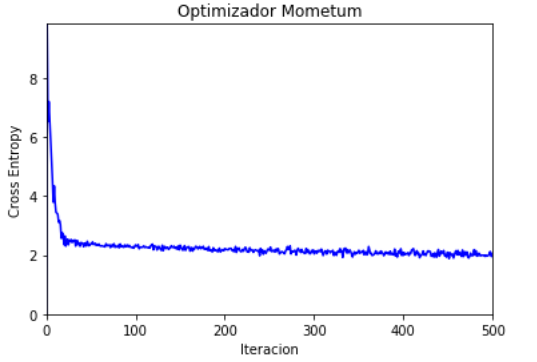
\includegraphics[width=0.5\textwidth]{Figures/momemtumcross5000.png}} 
		\subfloat[fig 2]{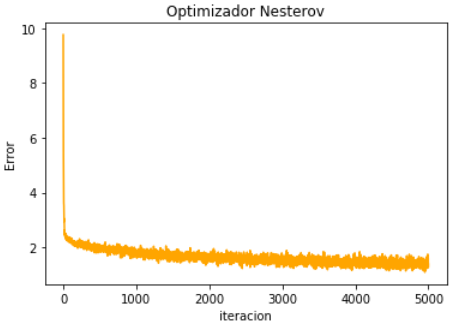
\includegraphics[width=0.5\textwidth]{Figures/nesterovcross5000.png}}\\
		\subfloat[fig 3]{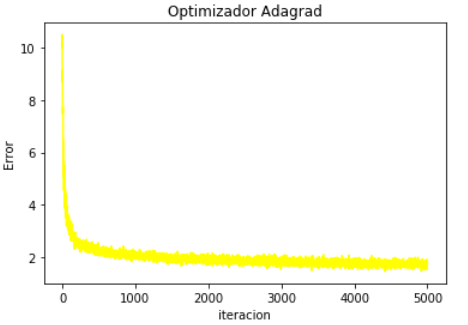
\includegraphics[width=0.5\textwidth]{Figures/adagradcross5000.png}}
		\subfloat[fig 3]{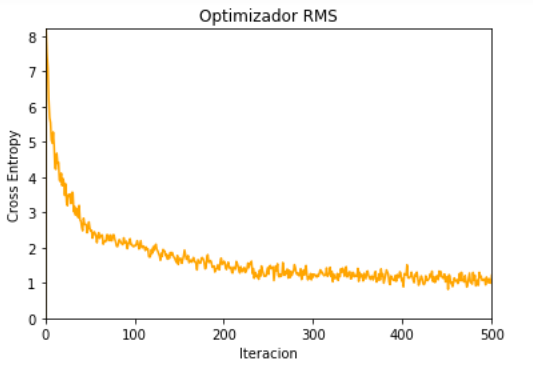
\includegraphics[width=0.5\textwidth]{Figures/rmscross5000.png}}\\
		\subfloat[fig 4]{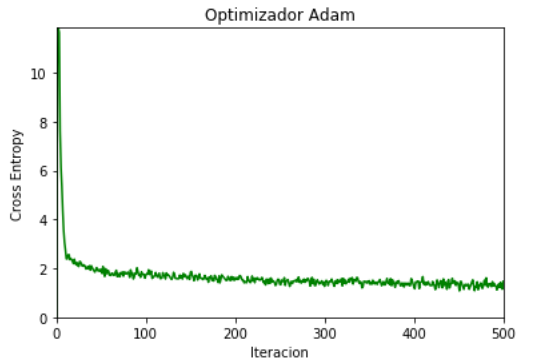
\includegraphics[width=0.5\textwidth]{Figures/adamcross5000.png}} 
		\caption{Error en los optimizadores 5000 epochs\\ Fuente:  \textit{Fuente Propia}}
		\label{some}
	\end{centering}
	
\end{figure}

\begin{figure}[H]
	\begin{centering}
		\subfloat[fig 1]{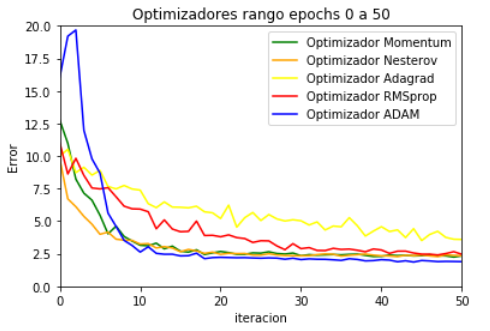
\includegraphics[width=0.8\textwidth]{Figures/optimizadorescross5000050}} 
		\caption{Comparación de las funciones de costo rango 0-50\\ Fuente:  \textit{Fuente Propia}}
		\label{some example5}
	\end{centering}
	
\end{figure}

\begin{figure}[H]
	\begin{centering}
		\subfloat[fig 1]{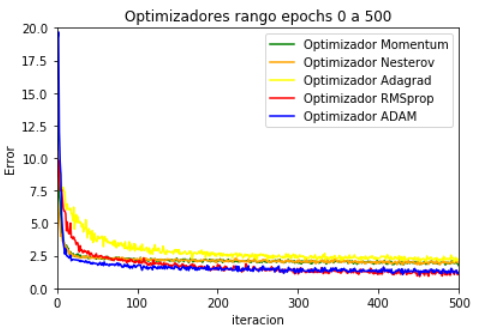
\includegraphics[width=0.8\textwidth]{Figures/optimizadorescross50000500}} 
		\caption{Comparación de las errores rango 0-500\\ Fuente:  \textit{Fuente Propia}}
		\label{some example6}
	\end{centering}
	
\end{figure}
\begin{figure}[H]
	\begin{centering}
		\subfloat[fig 1]{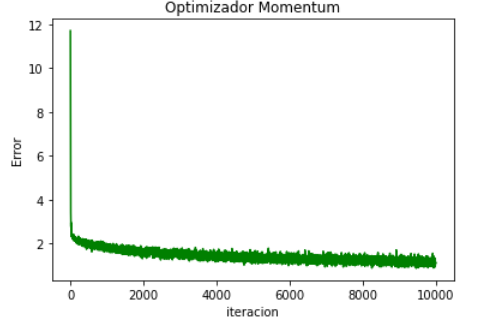
\includegraphics[width=0.6\textwidth]{Figures/momemtumcross10000.png}} 
		\subfloat[fig 2]{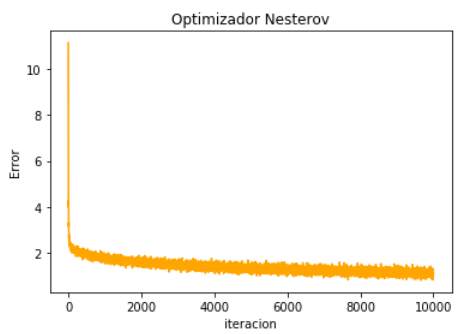
\includegraphics[width=0.6\textwidth]{Figures/nesterovcross10000.png}}\\
		\subfloat[fig 3]{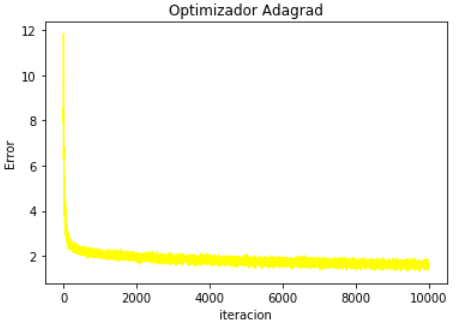
\includegraphics[width=0.6\textwidth]{Figures/adagradcross10000.png}}
		\subfloat[fig 3]{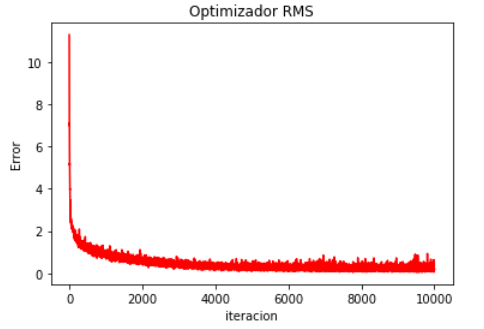
\includegraphics[width=0.6\textwidth]{Figures/RMScross10000.png}}\\
		\subfloat[fig 4]{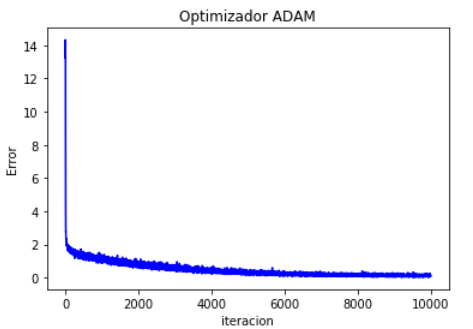
\includegraphics[width=0.6\textwidth]{Figures/adamcross10000.png}} 
		\caption{Error en los optimizadores 10000 epochs -CIFAR10\\ Fuente:  \textit{Fuente Propia}}

	\end{centering}
	
\end{figure}

\subsection{CIFAR-100}
\begin{figure}[H]
	\begin{centering}
		\subfloat[fig 1]{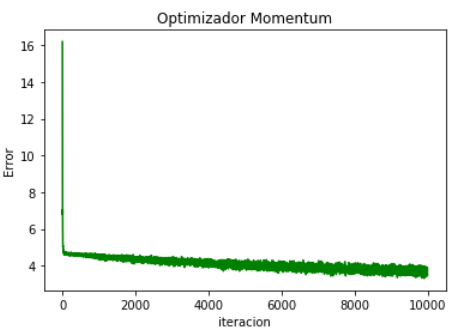
\includegraphics[width=0.6\textwidth]{Figures/100momentumcross10000.png}} 
		\subfloat[fig 2]{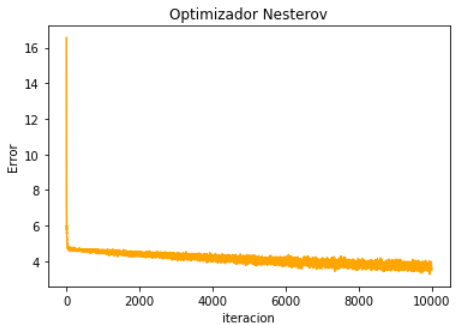
\includegraphics[width=0.6\textwidth]{Figures/100nesterovcross10000.png}}\\
		\subfloat[fig 3]{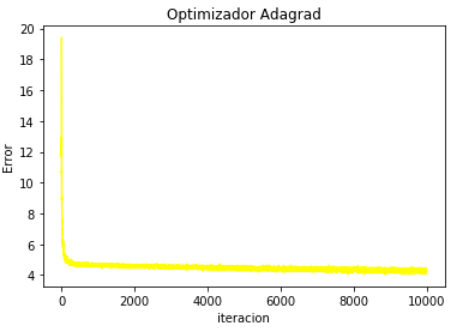
\includegraphics[width=0.6\textwidth]{Figures/100adagradcross10000.png}}
		\subfloat[fig 3]{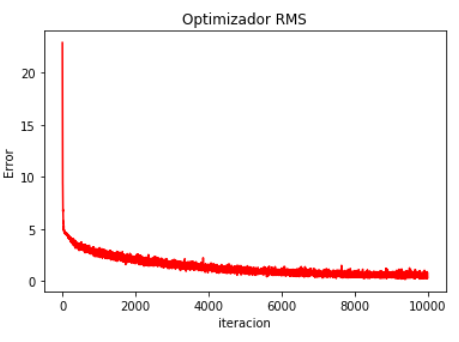
\includegraphics[width=0.6\textwidth]{Figures/100rmscross10000.png}}\\
		\subfloat[fig 4]{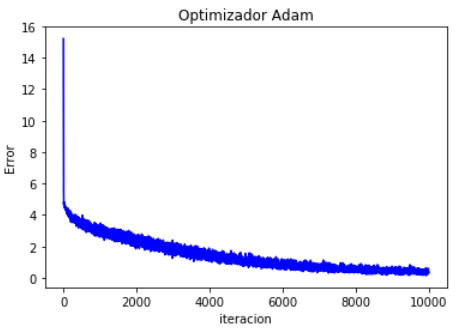
\includegraphics[width=0.6\textwidth]{Figures/100adamcross10000.png}} 
		\caption{Error en los optimizadores con 10000 epochs - CIFAR 100 \\ Fuente:  \textit{Fuente Propia}}
		\label{some2341}
	\end{centering}
	
\end{figure}

\begin{figure}[H]
	\begin{centering}
		\subfloat[fig 1]{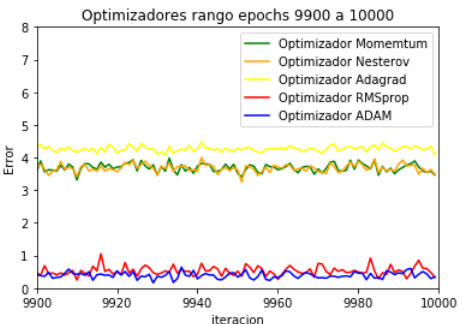
\includegraphics[width=0.8\textwidth]{Figures/cifar100error.png}} 
		\caption{Comparación los errores rango 9900-10000\\ Fuente:  \textit{Fuente Propia}}
		\label{COMPARACION}
	\end{centering}
	
\end{figure}
